\documentclass[twoside]{book}

% Packages required by doxygen
\usepackage{fixltx2e}
\usepackage{calc}
\usepackage{doxygen}
\usepackage[export]{adjustbox} % also loads graphicx
\usepackage{graphicx}
\usepackage[utf8]{inputenc}
\usepackage{makeidx}
\usepackage{multicol}
\usepackage{multirow}
\PassOptionsToPackage{warn}{textcomp}
\usepackage{textcomp}
\usepackage[nointegrals]{wasysym}
\usepackage[table]{xcolor}

% Font selection
\usepackage[T1]{fontenc}
\usepackage[scaled=.90]{helvet}
\usepackage{courier}
\usepackage{amssymb}
\usepackage{sectsty}
\renewcommand{\familydefault}{\sfdefault}
\allsectionsfont{%
  \fontseries{bc}\selectfont%
  \color{darkgray}%
}
\renewcommand{\DoxyLabelFont}{%
  \fontseries{bc}\selectfont%
  \color{darkgray}%
}
\newcommand{\+}{\discretionary{\mbox{\scriptsize$\hookleftarrow$}}{}{}}

% Page & text layout
\usepackage{geometry}
\geometry{%
  a4paper,%
  top=2.5cm,%
  bottom=2.5cm,%
  left=2.5cm,%
  right=2.5cm%
}
\tolerance=750
\hfuzz=15pt
\hbadness=750
\setlength{\emergencystretch}{15pt}
\setlength{\parindent}{0cm}
\setlength{\parskip}{3ex plus 2ex minus 2ex}
\makeatletter
\renewcommand{\paragraph}{%
  \@startsection{paragraph}{4}{0ex}{-1.0ex}{1.0ex}{%
    \normalfont\normalsize\bfseries\SS@parafont%
  }%
}
\renewcommand{\subparagraph}{%
  \@startsection{subparagraph}{5}{0ex}{-1.0ex}{1.0ex}{%
    \normalfont\normalsize\bfseries\SS@subparafont%
  }%
}
\makeatother

% Headers & footers
\usepackage{fancyhdr}
\pagestyle{fancyplain}
\fancyhead[LE]{\fancyplain{}{\bfseries\thepage}}
\fancyhead[CE]{\fancyplain{}{}}
\fancyhead[RE]{\fancyplain{}{\bfseries\leftmark}}
\fancyhead[LO]{\fancyplain{}{\bfseries\rightmark}}
\fancyhead[CO]{\fancyplain{}{}}
\fancyhead[RO]{\fancyplain{}{\bfseries\thepage}}
\fancyfoot[LE]{\fancyplain{}{}}
\fancyfoot[CE]{\fancyplain{}{}}
\fancyfoot[RE]{\fancyplain{}{\bfseries\scriptsize Generated by Doxygen }}
\fancyfoot[LO]{\fancyplain{}{\bfseries\scriptsize Generated by Doxygen }}
\fancyfoot[CO]{\fancyplain{}{}}
\fancyfoot[RO]{\fancyplain{}{}}
\renewcommand{\footrulewidth}{0.4pt}
\renewcommand{\chaptermark}[1]{%
  \markboth{#1}{}%
}
\renewcommand{\sectionmark}[1]{%
  \markright{\thesection\ #1}%
}

% Indices & bibliography
\usepackage{natbib}
\usepackage[titles]{tocloft}
\setcounter{tocdepth}{3}
\setcounter{secnumdepth}{5}
\makeindex

% Hyperlinks (required, but should be loaded last)
\usepackage{ifpdf}
\ifpdf
  \usepackage[pdftex,pagebackref=true]{hyperref}
\else
  \usepackage[ps2pdf,pagebackref=true]{hyperref}
\fi
\hypersetup{%
  colorlinks=true,%
  linkcolor=blue,%
  citecolor=blue,%
  unicode%
}

% Custom commands
\newcommand{\clearemptydoublepage}{%
  \newpage{\pagestyle{empty}\cleardoublepage}%
}

\usepackage{caption}
\captionsetup{labelsep=space,justification=centering,font={bf},singlelinecheck=off,skip=4pt,position=top}

%===== C O N T E N T S =====

\begin{document}

% Titlepage & ToC
\hypersetup{pageanchor=false,
             bookmarksnumbered=true,
             pdfencoding=unicode
            }
\pagenumbering{roman}
\begin{titlepage}
\vspace*{7cm}
\begin{center}%
{\Large Heisprosjekt }\\
\vspace*{1cm}
{\large Generated by Doxygen 1.8.11}\\
\end{center}
\end{titlepage}
\clearemptydoublepage
\tableofcontents
\clearemptydoublepage
\pagenumbering{arabic}
\hypersetup{pageanchor=true}

%--- Begin generated contents ---
\chapter{File Index}
\section{File List}
Here is a list of all documented files with brief descriptions\+:\begin{DoxyCompactList}
\item\contentsline{section}{source/{\bfseries channels.\+h} }{\pageref{channels_8h}}{}
\item\contentsline{section}{source/{\bfseries elev.\+c} }{\pageref{elev_8c}}{}
\item\contentsline{section}{source/\hyperlink{elev_8h}{elev.\+h} \\*A library containing functions regarding the elev (elevator) module }{\pageref{elev_8h}}{}
\item\contentsline{section}{source/{\bfseries F\+S\+M.\+c} }{\pageref{FSM_8c}}{}
\item\contentsline{section}{source/\hyperlink{FSM_8h}{F\+S\+M.\+h} \\*A library containing functions regarding the F\+SM (Finite-\/state machine) module }{\pageref{FSM_8h}}{}
\item\contentsline{section}{source/{\bfseries io.\+c} }{\pageref{io_8c}}{}
\item\contentsline{section}{source/\hyperlink{io_8h}{io.\+h} \\*A library containing functions regarding the io (in/out) module }{\pageref{io_8h}}{}
\item\contentsline{section}{source/{\bfseries lights.\+c} }{\pageref{lights_8c}}{}
\item\contentsline{section}{source/\hyperlink{lights_8h}{lights.\+h} \\*A library containing the functions regarding the lights module }{\pageref{lights_8h}}{}
\item\contentsline{section}{source/\hyperlink{main_8c}{main.\+c} \\*File for the main function of the program }{\pageref{main_8c}}{}
\item\contentsline{section}{source/{\bfseries queue.\+c} }{\pageref{queue_8c}}{}
\item\contentsline{section}{source/\hyperlink{queue_8h}{queue.\+h} \\*A library containing functions regarding the queue module }{\pageref{queue_8h}}{}
\item\contentsline{section}{source/{\bfseries timer.\+c} }{\pageref{timer_8c}}{}
\item\contentsline{section}{source/\hyperlink{timer_8h}{timer.\+h} \\*A library containing functions regarding the timer module }{\pageref{timer_8h}}{}
\end{DoxyCompactList}

\chapter{File Documentation}
\hypertarget{elev_8h}{}\section{source/elev.h File Reference}
\label{elev_8h}\index{source/elev.\+h@{source/elev.\+h}}


A library containing functions regarding the elev (elevator) module.  


This graph shows which files directly or indirectly include this file\+:

\hypertarget{FSM_8h}{}\section{source/\+F\+SM.h File Reference}
\label{FSM_8h}\index{source/\+F\+S\+M.\+h@{source/\+F\+S\+M.\+h}}


A library containing functions regarding the F\+SM (Finite-\/state machine) module.  


This graph shows which files directly or indirectly include this file\+:
\nopagebreak
\begin{figure}[H]
\begin{center}
\leavevmode
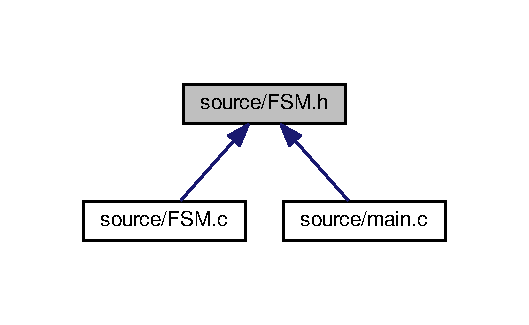
\includegraphics[width=254pt]{FSM_8h__dep__incl}
\end{center}
\end{figure}
\subsection*{Functions}
\begin{DoxyCompactItemize}
\item 
void \hyperlink{FSM_8h_a6e0568e2069dc494c5c9014a396b3900}{F\+S\+M\+\_\+state\+\_\+machine} ()\hypertarget{FSM_8h_a6e0568e2069dc494c5c9014a396b3900}{}\label{FSM_8h_a6e0568e2069dc494c5c9014a396b3900}

\begin{DoxyCompactList}\small\item\em Updates current state of the elevator and executes operations accordingly. \end{DoxyCompactList}\item 
int \hyperlink{FSM_8h_a5e55d574485ebc87b5d5a74a1a4b35e0}{F\+S\+M\+\_\+system\+\_\+init} ()
\begin{DoxyCompactList}\small\item\em Initializes hardware and leads the elevator to a defined state and position. \end{DoxyCompactList}\end{DoxyCompactItemize}


\subsection{Detailed Description}
A library containing functions regarding the F\+SM (Finite-\/state machine) module. 



\subsection{Function Documentation}
\index{F\+S\+M.\+h@{F\+S\+M.\+h}!F\+S\+M\+\_\+system\+\_\+init@{F\+S\+M\+\_\+system\+\_\+init}}
\index{F\+S\+M\+\_\+system\+\_\+init@{F\+S\+M\+\_\+system\+\_\+init}!F\+S\+M.\+h@{F\+S\+M.\+h}}
\subsubsection[{\texorpdfstring{F\+S\+M\+\_\+system\+\_\+init()}{FSM_system_init()}}]{\setlength{\rightskip}{0pt plus 5cm}int F\+S\+M\+\_\+system\+\_\+init (
\begin{DoxyParamCaption}
{}
\end{DoxyParamCaption}
)}\hypertarget{FSM_8h_a5e55d574485ebc87b5d5a74a1a4b35e0}{}\label{FSM_8h_a5e55d574485ebc87b5d5a74a1a4b35e0}


Initializes hardware and leads the elevator to a defined state and position. 

\begin{DoxyReturn}{Returns}
0 if the elevator hardware is unable to initialize, 1 otherwise. 
\end{DoxyReturn}


Definition at line 46 of file F\+S\+M.\+c.


\hypertarget{io_8h}{}\section{source/io.h File Reference}
\label{io_8h}\index{source/io.\+h@{source/io.\+h}}


A library containing functions regarding the io (in/out) module.  


This graph shows which files directly or indirectly include this file\+:
% FIG 0
\subsection*{Functions}
\begin{DoxyCompactItemize}
\item 
int \hyperlink{io_8h_a12ce98b64f2019ac45b44826a4db7ec9}{io\+\_\+init} ()
\item 
void \hyperlink{io_8h_a4d538858b80ee856217e3ecfde8a3c60}{io\+\_\+set\+\_\+bit} (int channel)
\item 
void \hyperlink{io_8h_a97951257634a0778b858a4ced7558f81}{io\+\_\+clear\+\_\+bit} (int channel)
\item 
void \hyperlink{io_8h_a1c2c5df63111187109ef11be354621bd}{io\+\_\+write\+\_\+analog} (int channel, int value)
\item 
int \hyperlink{io_8h_ae9e08ee7d41b07b153e2ddaae4dc53cb}{io\+\_\+read\+\_\+bit} (int channel)
\item 
int \hyperlink{io_8h_ab145a5637d2c463dfb5741e1a748dd74}{io\+\_\+read\+\_\+analog} (int channel)
\end{DoxyCompactItemize}


\subsection{Detailed Description}
A library containing functions regarding the io (in/out) module. 



\subsection{Function Documentation}
\index{io.\+h@{io.\+h}!io\+\_\+clear\+\_\+bit@{io\+\_\+clear\+\_\+bit}}
\index{io\+\_\+clear\+\_\+bit@{io\+\_\+clear\+\_\+bit}!io.\+h@{io.\+h}}
\subsubsection[{\texorpdfstring{io\+\_\+clear\+\_\+bit(int channel)}{io_clear_bit(int channel)}}]{\setlength{\rightskip}{0pt plus 5cm}void io\+\_\+clear\+\_\+bit (
\begin{DoxyParamCaption}
\item[{int}]{channel}
\end{DoxyParamCaption}
)}\hypertarget{io_8h_a97951257634a0778b858a4ced7558f81}{}\label{io_8h_a97951257634a0778b858a4ced7558f81}
Clears a digital channel bit. 
\begin{DoxyParams}{Parameters}
{\em channel} & Channel bit to set. \\
\hline
\end{DoxyParams}


Definition at line 45 of file io.\+c.

\index{io.\+h@{io.\+h}!io\+\_\+init@{io\+\_\+init}}
\index{io\+\_\+init@{io\+\_\+init}!io.\+h@{io.\+h}}
\subsubsection[{\texorpdfstring{io\+\_\+init()}{io_init()}}]{\setlength{\rightskip}{0pt plus 5cm}int io\+\_\+init (
\begin{DoxyParamCaption}
{}
\end{DoxyParamCaption}
)}\hypertarget{io_8h_a12ce98b64f2019ac45b44826a4db7ec9}{}\label{io_8h_a12ce98b64f2019ac45b44826a4db7ec9}
Initialize lib\+Comedi in \char`\"{}\+Sanntidssalen\char`\"{} \begin{DoxyReturn}{Returns}
Non-\/zero on success and 0 on failure 
\end{DoxyReturn}


Definition at line 18 of file io.\+c.

\index{io.\+h@{io.\+h}!io\+\_\+read\+\_\+analog@{io\+\_\+read\+\_\+analog}}
\index{io\+\_\+read\+\_\+analog@{io\+\_\+read\+\_\+analog}!io.\+h@{io.\+h}}
\subsubsection[{\texorpdfstring{io\+\_\+read\+\_\+analog(int channel)}{io_read_analog(int channel)}}]{\setlength{\rightskip}{0pt plus 5cm}int io\+\_\+read\+\_\+analog (
\begin{DoxyParamCaption}
\item[{int}]{channel}
\end{DoxyParamCaption}
)}\hypertarget{io_8h_ab145a5637d2c463dfb5741e1a748dd74}{}\label{io_8h_ab145a5637d2c463dfb5741e1a748dd74}
Reads a bit value from an analog channel. 
\begin{DoxyParams}{Parameters}
{\em channel} & Channel to read from. \\
\hline
\end{DoxyParams}
\begin{DoxyReturn}{Returns}
Value read. 
\end{DoxyReturn}


Definition at line 66 of file io.\+c.

\index{io.\+h@{io.\+h}!io\+\_\+read\+\_\+bit@{io\+\_\+read\+\_\+bit}}
\index{io\+\_\+read\+\_\+bit@{io\+\_\+read\+\_\+bit}!io.\+h@{io.\+h}}
\subsubsection[{\texorpdfstring{io\+\_\+read\+\_\+bit(int channel)}{io_read_bit(int channel)}}]{\setlength{\rightskip}{0pt plus 5cm}int io\+\_\+read\+\_\+bit (
\begin{DoxyParamCaption}
\item[{int}]{channel}
\end{DoxyParamCaption}
)}\hypertarget{io_8h_ae9e08ee7d41b07b153e2ddaae4dc53cb}{}\label{io_8h_ae9e08ee7d41b07b153e2ddaae4dc53cb}
Reads a bit value from a digital channel. 
\begin{DoxyParams}{Parameters}
{\em channel} & Channel to read from. \\
\hline
\end{DoxyParams}
\begin{DoxyReturn}{Returns}
Value read. 
\end{DoxyReturn}


Definition at line 57 of file io.\+c.

\index{io.\+h@{io.\+h}!io\+\_\+set\+\_\+bit@{io\+\_\+set\+\_\+bit}}
\index{io\+\_\+set\+\_\+bit@{io\+\_\+set\+\_\+bit}!io.\+h@{io.\+h}}
\subsubsection[{\texorpdfstring{io\+\_\+set\+\_\+bit(int channel)}{io_set_bit(int channel)}}]{\setlength{\rightskip}{0pt plus 5cm}void io\+\_\+set\+\_\+bit (
\begin{DoxyParamCaption}
\item[{int}]{channel}
\end{DoxyParamCaption}
)}\hypertarget{io_8h_a4d538858b80ee856217e3ecfde8a3c60}{}\label{io_8h_a4d538858b80ee856217e3ecfde8a3c60}
Sets a digital channel bit. 
\begin{DoxyParams}{Parameters}
{\em channel} & Channel bit to set. \\
\hline
\end{DoxyParams}


Definition at line 39 of file io.\+c.

\index{io.\+h@{io.\+h}!io\+\_\+write\+\_\+analog@{io\+\_\+write\+\_\+analog}}
\index{io\+\_\+write\+\_\+analog@{io\+\_\+write\+\_\+analog}!io.\+h@{io.\+h}}
\subsubsection[{\texorpdfstring{io\+\_\+write\+\_\+analog(int channel, int value)}{io_write_analog(int channel, int value)}}]{\setlength{\rightskip}{0pt plus 5cm}void io\+\_\+write\+\_\+analog (
\begin{DoxyParamCaption}
\item[{int}]{channel, }
\item[{int}]{value}
\end{DoxyParamCaption}
)}\hypertarget{io_8h_a1c2c5df63111187109ef11be354621bd}{}\label{io_8h_a1c2c5df63111187109ef11be354621bd}
Writes a value to an analog channel. 
\begin{DoxyParams}{Parameters}
{\em channel} & Channel to write to. \\
\hline
{\em value} & Value to write. \\
\hline
\end{DoxyParams}


Definition at line 51 of file io.\+c.


\hypertarget{lights_8h}{}\section{source/lights.h File Reference}
\label{lights_8h}\index{source/lights.\+h@{source/lights.\+h}}


A library containing the functions regarding the lights module.  


{\ttfamily \#include \char`\"{}elev.\+h\char`\"{}}\\*
Include dependency graph for lights.\+h\+:\nopagebreak
\begin{figure}[H]
\begin{center}
\leavevmode
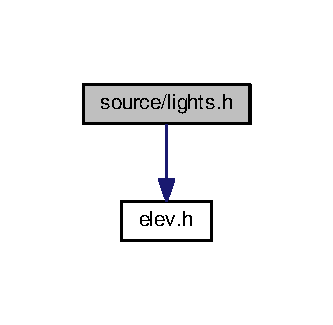
\includegraphics[width=160pt]{lights_8h__incl}
\end{center}
\end{figure}
This graph shows which files directly or indirectly include this file\+:\nopagebreak
\begin{figure}[H]
\begin{center}
\leavevmode
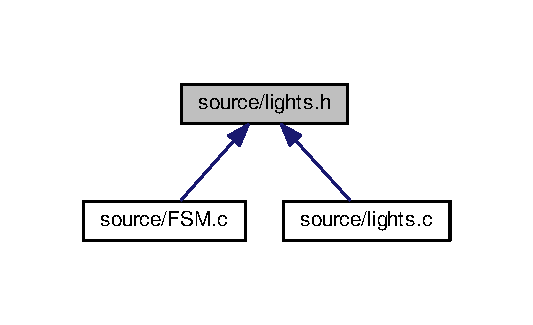
\includegraphics[width=256pt]{lights_8h__dep__incl}
\end{center}
\end{figure}
\subsection*{Functions}
\begin{DoxyCompactItemize}
\item 
void \hyperlink{lights_8h_af2210991bdfe739662bce1dd46388d27}{lights\+\_\+update\+\_\+ordering\+\_\+lights} ()\hypertarget{lights_8h_af2210991bdfe739662bce1dd46388d27}{}\label{lights_8h_af2210991bdfe739662bce1dd46388d27}

\begin{DoxyCompactList}\small\item\em Updates the ordering lights, on or off, according to the array \char`\"{}lights\char`\"{}. \end{DoxyCompactList}\item 
void \hyperlink{lights_8h_a9581cca0e3b21bb9db5d4dac1f5d04fd}{lights\+\_\+reset\+\_\+ordering\+\_\+lights\+\_\+array} (int floor)
\begin{DoxyCompactList}\small\item\em Sets the values in the array \char`\"{}lights\char`\"{} for the ordering lights to the corresponding floor to 0. \end{DoxyCompactList}\item 
void \hyperlink{lights_8h_ab9e40612b431e6952a2b51b6b20c6843}{lights\+\_\+reset\+\_\+all\+\_\+ordering\+\_\+lights\+\_\+array} ()\hypertarget{lights_8h_ab9e40612b431e6952a2b51b6b20c6843}{}\label{lights_8h_ab9e40612b431e6952a2b51b6b20c6843}

\begin{DoxyCompactList}\small\item\em Sets all the values in the array \char`\"{}lights\char`\"{} to 0. \end{DoxyCompactList}\item 
void \hyperlink{lights_8h_ab9fdad0624f78e12a34b9aed0e501604}{lights\+\_\+set\+\_\+ordering\+\_\+lights\+\_\+array} ()\hypertarget{lights_8h_ab9fdad0624f78e12a34b9aed0e501604}{}\label{lights_8h_ab9fdad0624f78e12a34b9aed0e501604}

\begin{DoxyCompactList}\small\item\em Gets signal from ordering button, and sets the corresponding element in the \char`\"{}lights\char`\"{} array to 1. \end{DoxyCompactList}\end{DoxyCompactItemize}


\subsection{Detailed Description}
A library containing the functions regarding the lights module. 



\subsection{Function Documentation}
\index{lights.\+h@{lights.\+h}!lights\+\_\+reset\+\_\+ordering\+\_\+lights\+\_\+array@{lights\+\_\+reset\+\_\+ordering\+\_\+lights\+\_\+array}}
\index{lights\+\_\+reset\+\_\+ordering\+\_\+lights\+\_\+array@{lights\+\_\+reset\+\_\+ordering\+\_\+lights\+\_\+array}!lights.\+h@{lights.\+h}}
\subsubsection[{\texorpdfstring{lights\+\_\+reset\+\_\+ordering\+\_\+lights\+\_\+array(int floor)}{lights_reset_ordering_lights_array(int floor)}}]{\setlength{\rightskip}{0pt plus 5cm}void lights\+\_\+reset\+\_\+ordering\+\_\+lights\+\_\+array (
\begin{DoxyParamCaption}
\item[{int}]{floor}
\end{DoxyParamCaption}
)}\hypertarget{lights_8h_a9581cca0e3b21bb9db5d4dac1f5d04fd}{}\label{lights_8h_a9581cca0e3b21bb9db5d4dac1f5d04fd}


Sets the values in the array \char`\"{}lights\char`\"{} for the ordering lights to the corresponding floor to 0. 


\begin{DoxyParams}[1]{Parameters}
\mbox{\tt in}  & {\em floor} & The floor where the ordering lights will be turned off. Must be an integer in range 0-\/3. \\
\hline
\end{DoxyParams}


Definition at line 46 of file lights.\+c.


\hypertarget{main_8c}{}\section{source/main.c File Reference}
\label{main_8c}\index{source/main.\+c@{source/main.\+c}}


File for the main function of the program.  


{\ttfamily \#include \char`\"{}F\+S\+M.\+h\char`\"{}}\\*
{\ttfamily \#include $<$stdio.\+h$>$}\\*
Include dependency graph for main.\+c\+:
% FIG 0
\subsection*{Functions}
\begin{DoxyCompactItemize}
\item 
int {\bfseries main} ()\hypertarget{main_8c_ae66f6b31b5ad750f1fe042a706a4e3d4}{}\label{main_8c_ae66f6b31b5ad750f1fe042a706a4e3d4}

\end{DoxyCompactItemize}


\subsection{Detailed Description}
File for the main function of the program. 


\hypertarget{queue_8h}{}\section{source/queue.h File Reference}
\label{queue_8h}\index{source/queue.\+h@{source/queue.\+h}}


A library containing functions regarding the queue module.  


{\ttfamily \#include \char`\"{}elev.\+h\char`\"{}}\\*
Include dependency graph for queue.\+h\+:
% FIG 0
This graph shows which files directly or indirectly include this file\+:
% FIG 1
\subsection*{Functions}
\begin{DoxyCompactItemize}
\item 
void \hyperlink{queue_8h_a35a940db362073d0e6f2de5c98ca8642}{queue\+\_\+take\+\_\+order} ()\hypertarget{queue_8h_a35a940db362073d0e6f2de5c98ca8642}{}\label{queue_8h_a35a940db362073d0e6f2de5c98ca8642}

\begin{DoxyCompactList}\small\item\em Sets the value in the array \char`\"{}orders\char`\"{} to the corresponding order to 1. \end{DoxyCompactList}\item 
int \hyperlink{queue_8h_a8db0e454b9930c5cd767d158d9e46ebc}{queue\+\_\+get\+\_\+order} (int floor)
\begin{DoxyCompactList}\small\item\em Checks if there are any orders to given floor. \end{DoxyCompactList}\item 
void \hyperlink{queue_8h_af136c602c4abb11df25cf6e362407e0f}{queue\+\_\+delete\+\_\+order} (int floor)
\begin{DoxyCompactList}\small\item\em Sets the value in the array \char`\"{}orders\char`\"{} to the corresponding order to 0. \end{DoxyCompactList}\item 
void \hyperlink{queue_8h_a25ddb5a68fbbd63e2ceb905b3c57595f}{queue\+\_\+delete\+\_\+all\+\_\+orders} ()\hypertarget{queue_8h_a25ddb5a68fbbd63e2ceb905b3c57595f}{}\label{queue_8h_a25ddb5a68fbbd63e2ceb905b3c57595f}

\begin{DoxyCompactList}\small\item\em Sets all values in the array \char`\"{}orders\char`\"{} to 0. \end{DoxyCompactList}\item 
\hyperlink{elev_8h_a2256dfd58fecce253106f83fd2ed607f}{elev\+\_\+motor\+\_\+direction\+\_\+t} \hyperlink{queue_8h_a1f7111dc281ee03f5e22553494e3c9c1}{queue\+\_\+calculate\+\_\+direction} (\hyperlink{elev_8h_a2256dfd58fecce253106f83fd2ed607f}{elev\+\_\+motor\+\_\+direction\+\_\+t} dir, int pos, int pos\+\_\+between)
\begin{DoxyCompactList}\small\item\em Calculates the elevator\textquotesingle{}s next direction. \end{DoxyCompactList}\item 
int \hyperlink{queue_8h_a9bda618087afe5dc6c669643b2628537}{queue\+\_\+should\+\_\+stop\+\_\+at\+\_\+floor} (\hyperlink{elev_8h_a2256dfd58fecce253106f83fd2ed607f}{elev\+\_\+motor\+\_\+direction\+\_\+t} motor\+\_\+dir, int floor)
\begin{DoxyCompactList}\small\item\em Checks if the elevator should stop at the given floor. \end{DoxyCompactList}\item 
int \hyperlink{queue_8h_a03cce911f28d999c0647e7ce9e928ff9}{queue\+\_\+have\+\_\+orders} ()
\begin{DoxyCompactList}\small\item\em Checks if there are any orders. \end{DoxyCompactList}\end{DoxyCompactItemize}


\subsection{Detailed Description}
A library containing functions regarding the queue module. 



\subsection{Function Documentation}
\index{queue.\+h@{queue.\+h}!queue\+\_\+calculate\+\_\+direction@{queue\+\_\+calculate\+\_\+direction}}
\index{queue\+\_\+calculate\+\_\+direction@{queue\+\_\+calculate\+\_\+direction}!queue.\+h@{queue.\+h}}
\subsubsection[{\texorpdfstring{queue\+\_\+calculate\+\_\+direction(elev\+\_\+motor\+\_\+direction\+\_\+t dir, int pos, int pos\+\_\+between)}{queue_calculate_direction(elev_motor_direction_t dir, int pos, int pos_between)}}]{\setlength{\rightskip}{0pt plus 5cm}{\bf elev\+\_\+motor\+\_\+direction\+\_\+t} queue\+\_\+calculate\+\_\+direction (
\begin{DoxyParamCaption}
\item[{{\bf elev\+\_\+motor\+\_\+direction\+\_\+t}}]{dir, }
\item[{int}]{pos, }
\item[{int}]{pos\+\_\+between}
\end{DoxyParamCaption}
)}\hypertarget{queue_8h_a1f7111dc281ee03f5e22553494e3c9c1}{}\label{queue_8h_a1f7111dc281ee03f5e22553494e3c9c1}


Calculates the elevator\textquotesingle{}s next direction. 


\begin{DoxyParams}[1]{Parameters}
\mbox{\tt in}  & {\em dir} & The direction of the elevator\textquotesingle{}s movement. Must have the following values\+: D\+I\+R\+N\+\_\+\+D\+O\+WN = -\/1, D\+I\+R\+N\+\_\+\+S\+T\+OP = 0 or D\+I\+R\+N\+\_\+\+UP = 1.\\
\hline
\mbox{\tt in}  & {\em pos} & Previous detected floor by sensor. Must be in range 0-\/3.\\
\hline
\mbox{\tt in}  & {\em pos\+\_\+between} & Keeps track of which floors the elevator is located between at any given time. Must be in range 1-\/3.\\
\hline
\end{DoxyParams}
\begin{DoxyReturn}{Returns}
D\+I\+R\+N\+\_\+\+D\+O\+WN = -\/1 when moving down. D\+I\+R\+N\+\_\+\+S\+T\+OP = 0 when stationary. D\+I\+R\+N\+\_\+\+UP = 1 when moving up. 
\end{DoxyReturn}


Definition at line 139 of file queue.\+c.

\index{queue.\+h@{queue.\+h}!queue\+\_\+delete\+\_\+order@{queue\+\_\+delete\+\_\+order}}
\index{queue\+\_\+delete\+\_\+order@{queue\+\_\+delete\+\_\+order}!queue.\+h@{queue.\+h}}
\subsubsection[{\texorpdfstring{queue\+\_\+delete\+\_\+order(int floor)}{queue_delete_order(int floor)}}]{\setlength{\rightskip}{0pt plus 5cm}void queue\+\_\+delete\+\_\+order (
\begin{DoxyParamCaption}
\item[{int}]{floor}
\end{DoxyParamCaption}
)}\hypertarget{queue_8h_af136c602c4abb11df25cf6e362407e0f}{}\label{queue_8h_af136c602c4abb11df25cf6e362407e0f}


Sets the value in the array \char`\"{}orders\char`\"{} to the corresponding order to 0. 


\begin{DoxyParams}[1]{Parameters}
\mbox{\tt in}  & {\em floor} & The floor where the function deletes the corresponding orders. Must be an integer in range 0-\/3. \\
\hline
\end{DoxyParams}


Definition at line 102 of file queue.\+c.

\index{queue.\+h@{queue.\+h}!queue\+\_\+get\+\_\+order@{queue\+\_\+get\+\_\+order}}
\index{queue\+\_\+get\+\_\+order@{queue\+\_\+get\+\_\+order}!queue.\+h@{queue.\+h}}
\subsubsection[{\texorpdfstring{queue\+\_\+get\+\_\+order(int floor)}{queue_get_order(int floor)}}]{\setlength{\rightskip}{0pt plus 5cm}int queue\+\_\+get\+\_\+order (
\begin{DoxyParamCaption}
\item[{int}]{floor}
\end{DoxyParamCaption}
)}\hypertarget{queue_8h_a8db0e454b9930c5cd767d158d9e46ebc}{}\label{queue_8h_a8db0e454b9930c5cd767d158d9e46ebc}


Checks if there are any orders to given floor. 


\begin{DoxyParams}[1]{Parameters}
\mbox{\tt in}  & {\em floor} & The floor where the function looks for orders. Must be an integer in range 0-\/3.\\
\hline
\end{DoxyParams}
\begin{DoxyReturn}{Returns}
1 if there is an order at floor {\ttfamily floor}. 0 otherwise. 
\end{DoxyReturn}


Definition at line 77 of file queue.\+c.

\index{queue.\+h@{queue.\+h}!queue\+\_\+have\+\_\+orders@{queue\+\_\+have\+\_\+orders}}
\index{queue\+\_\+have\+\_\+orders@{queue\+\_\+have\+\_\+orders}!queue.\+h@{queue.\+h}}
\subsubsection[{\texorpdfstring{queue\+\_\+have\+\_\+orders()}{queue_have_orders()}}]{\setlength{\rightskip}{0pt plus 5cm}int queue\+\_\+have\+\_\+orders (
\begin{DoxyParamCaption}
{}
\end{DoxyParamCaption}
)}\hypertarget{queue_8h_a03cce911f28d999c0647e7ce9e928ff9}{}\label{queue_8h_a03cce911f28d999c0647e7ce9e928ff9}


Checks if there are any orders. 

\begin{DoxyReturn}{Returns}
1 if there are any orders. 0 otherwise. 
\end{DoxyReturn}


Definition at line 190 of file queue.\+c.

\index{queue.\+h@{queue.\+h}!queue\+\_\+should\+\_\+stop\+\_\+at\+\_\+floor@{queue\+\_\+should\+\_\+stop\+\_\+at\+\_\+floor}}
\index{queue\+\_\+should\+\_\+stop\+\_\+at\+\_\+floor@{queue\+\_\+should\+\_\+stop\+\_\+at\+\_\+floor}!queue.\+h@{queue.\+h}}
\subsubsection[{\texorpdfstring{queue\+\_\+should\+\_\+stop\+\_\+at\+\_\+floor(elev\+\_\+motor\+\_\+direction\+\_\+t motor\+\_\+dir, int floor)}{queue_should_stop_at_floor(elev_motor_direction_t motor_dir, int floor)}}]{\setlength{\rightskip}{0pt plus 5cm}int queue\+\_\+should\+\_\+stop\+\_\+at\+\_\+floor (
\begin{DoxyParamCaption}
\item[{{\bf elev\+\_\+motor\+\_\+direction\+\_\+t}}]{motor\+\_\+dir, }
\item[{int}]{floor}
\end{DoxyParamCaption}
)}\hypertarget{queue_8h_a9bda618087afe5dc6c669643b2628537}{}\label{queue_8h_a9bda618087afe5dc6c669643b2628537}


Checks if the elevator should stop at the given floor. 


\begin{DoxyParams}[1]{Parameters}
\mbox{\tt in}  & {\em motor\+\_\+dir} & The direction of the elevator\textquotesingle{}s movement. Must have the following values\+: D\+I\+R\+N\+\_\+\+D\+O\+WN = -\/1, D\+I\+R\+N\+\_\+\+S\+T\+OP = 0 or D\+I\+R\+N\+\_\+\+UP = 1.\\
\hline
\mbox{\tt in}  & {\em floor} & The floor where the function checks if it should stop. Must be an integer in range 0-\/3.\\
\hline
\end{DoxyParams}
\begin{DoxyReturn}{Returns}
1 if elevator should stop. 0 otherwise. 
\end{DoxyReturn}


Definition at line 168 of file queue.\+c.


\hypertarget{timer_8h}{}\section{source/timer.h File Reference}
\label{timer_8h}\index{source/timer.\+h@{source/timer.\+h}}


A library containing functions regarding the timer module.  


{\ttfamily \#include $<$time.\+h$>$}\\*
Include dependency graph for timer.\+h\+:\nopagebreak
\begin{figure}[H]
\begin{center}
\leavevmode
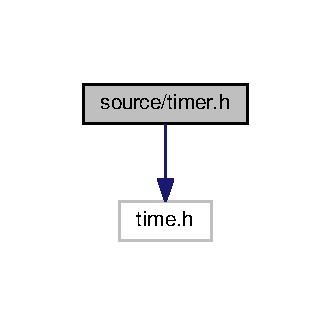
\includegraphics[width=159pt]{timer_8h__incl}
\end{center}
\end{figure}
This graph shows which files directly or indirectly include this file\+:\nopagebreak
\begin{figure}[H]
\begin{center}
\leavevmode
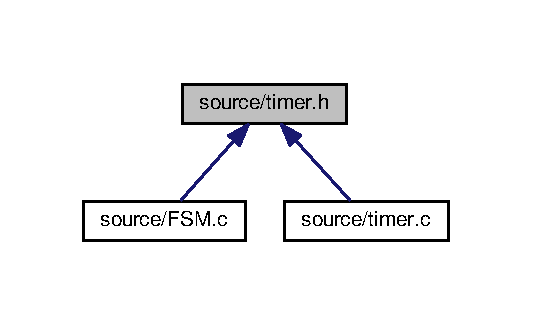
\includegraphics[width=256pt]{timer_8h__dep__incl}
\end{center}
\end{figure}
\subsection*{Functions}
\begin{DoxyCompactItemize}
\item 
void \hyperlink{timer_8h_a7f1ca02cbf81adb4494ece96457c6c5f}{timer\+\_\+reset} ()\hypertarget{timer_8h_a7f1ca02cbf81adb4494ece96457c6c5f}{}\label{timer_8h_a7f1ca02cbf81adb4494ece96457c6c5f}

\begin{DoxyCompactList}\small\item\em Sets a new timestamp. \end{DoxyCompactList}\item 
int \hyperlink{timer_8h_aa407a36b99e4dd9072e1fb40c1d793d0}{timer\+\_\+expired} ()
\begin{DoxyCompactList}\small\item\em Checks if it has been more than T\+I\+M\+E\+\_\+\+L\+I\+M\+IT secounds since last timstamp. \end{DoxyCompactList}\end{DoxyCompactItemize}


\subsection{Detailed Description}
A library containing functions regarding the timer module. 



\subsection{Function Documentation}
\index{timer.\+h@{timer.\+h}!timer\+\_\+expired@{timer\+\_\+expired}}
\index{timer\+\_\+expired@{timer\+\_\+expired}!timer.\+h@{timer.\+h}}
\subsubsection[{\texorpdfstring{timer\+\_\+expired()}{timer_expired()}}]{\setlength{\rightskip}{0pt plus 5cm}int timer\+\_\+expired (
\begin{DoxyParamCaption}
{}
\end{DoxyParamCaption}
)}\hypertarget{timer_8h_aa407a36b99e4dd9072e1fb40c1d793d0}{}\label{timer_8h_aa407a36b99e4dd9072e1fb40c1d793d0}


Checks if it has been more than T\+I\+M\+E\+\_\+\+L\+I\+M\+IT secounds since last timstamp. 

\begin{DoxyReturn}{Returns}
1 if the time limit has surpassed. 0 otherwise. 
\end{DoxyReturn}


Definition at line 27 of file timer.\+c.


%--- End generated contents ---

% Index
\backmatter
\newpage
\phantomsection
\clearemptydoublepage
\addcontentsline{toc}{chapter}{Index}
\printindex

\end{document}
